% 
% Annual Cognitive Science Conference
% Sample LaTeX Paper -- Proceedings Format
% 

% Original : Ashwin Ram (ashwin@cc.gatech.edu)       04/01/1994
% Modified : Johanna Moore (jmoore@cs.pitt.edu)      03/17/1995
% Modified : David Noelle (noelle@ucsd.edu)          03/15/1996
% Modified : Pat Langley (langley@cs.stanford.edu)   01/26/1997
% Latex2e corrections by Ramin Charles Nakisa        01/28/1997 
% Modified : Tina Eliassi-Rad (eliassi@cs.wisc.edu)  01/31/1998
% Modified : Trisha Yannuzzi (trisha@ircs.upenn.edu) 12/28/1999 (in process)
% Modified : Mary Ellen Foster (M.E.Foster@ed.ac.uk) 12/11/2000
% Modified : Ken Forbus                              01/23/2004
% Modified : Eli M. Silk (esilk@pitt.edu)            05/24/2005
% Modified: Niels Taatgen (taatgen@cmu.edu)  10/24/2006

%% Change ``a4paper'' in the following line to ``letterpaper'' if you are
%% producing a letter-format document.






%%%% Remaining todos
% overall proofreading


% illusory control over OUTCOME closeness vs. actual control over number or position


\documentclass[10pt,letterpaper]{article}

\usepackage{cogsci}
\usepackage{pslatex}
\usepackage{apacite}
\usepackage{graphicx}
\usepackage{color}
\usepackage{amsmath}
\usepackage{multirow}
\usepackage{amssymb}
%\usepackage{url}
%\usepackage{hyperref}


 
\definecolor{Red}{RGB}{255,0,0}
\newcommand{\red}[1]{\textcolor{Red}{#1}}  

%When does a near-miss sting?
%When does close count?
%When closeness counts: ...
%I was so close!
% He was soooo close! Near-misses hurt in random events

% Near-misses hurt even in games of chance
% a near miss stings even when it's random and uncontrollable
\title{ Near-misses sting even when they are uncontrollable }
 
\author{{\large \bf Desmond C. Ong (dco@stanford.edu)} \\
{\large \bf Noah D. Goodman (ngoodman@stanford.edu)} \\
{\large \bf Jamil Zaki (jzaki@stanford.edu)} \\
  Department of Psychology, Stanford University, Stanford CA, USA 
}

\begin{document}

\maketitle

\begin{abstract}
Observers often judge agents who miss a desired outcome by a small, compared to a large, margin to be less happy. This \textit{near-miss effect} has typically been examined in situations where the agents have control over outcomes (e.g., missing a flight). Here, we extend this work in three ways.  First, we show that near-miss effects play into observers' intuitive theories of emotion even for randomly-determined outcomes over which agents demonstrably have no control.  Second, we find data consistent with a hypothesis in which---even in randomly determined cases---near-miss effects reflect an \textit{illusion of control} over those events. Finally, we integrate near-miss effects into a broader model of affective cognition, and quantify the psychological cost of a missing a desired outcome by relatively little distance, relative to winning or losing that outcome.

\textbf{Keywords:} 
Near-Miss; Counterfactual Distance; Lay Theories; Emotion; Illusory Control
\end{abstract}


\begin{quote}
\textit{``Close only counts in horseshoes and hand grenades"} 
--- English Proverb
\end{quote}


	Observers typically infer that people feel more positively when they succeed, rather than fail, at attaining desired outcomes (e.g., winning vs. losing a soccer game). Such intuitive reasoning about emotions comprises what we term \textit{affective cognition} \cite{OngAffCog}, and forms an integral part of our social lives. Our intuitive theories of emotion, however, are more nuanced than simple considerations of success and failure: If an agent fails to achieve an outcome by a small margin, such as losing a soccer game by a single goal (\textit{a near-miss}), people often infer that the agent would feel worse than if they had lost by a larger margin. Penalty shootouts in soccer provides the most exaggerated of such near-miss scenarios: the losing team often loses because of a single shot, sometimes an inch shy of escaping the goalkeeper's hands. In cases like these, contrary to the proverb above, close \textit{does} count---\textit{emotionally}.


	Psychologists have long examined near-misses \cite{Gleicher1990, Johnson1986, Kahneman1982, Teigen1996}, but have yet to factor them systematically into theories of reasoning about emotions \cite{OngAffCog}. Most of this work examines counterfactual thinking more broadly, or thinking about ``what might have been" \cite{Bryne2002,McMullen2002, Medvec1997, Roese1997}. On most accounts, near-misses increase counterfactual thinking, because alternate outcomes almost occurred, and thus are easier to imagine. 


	Many open questions remain regarding the nature of near-miss effects, and how they impact observers' lay theories of emotion. First, when and why do people infer that a near-miss will ``hurt" an agent most? One explanation is that agents experiencing a near-miss could have done something different to achieve the desired outcome, increasing their subsequent experience of regret \cite<e.g.,>{Zeelenberg1998}.  Consider \citeA{Kahneman1982}'s classic example of Mr. Tees, who missed his plane by 5 minutes, and Mr. Crane, who missed his plane by 30 minutes. People reliably judge Mr. Tees, who narrowly missed his plane, to feel worse than Mr. Crane. Here, Mr. Tees could have left his home slightly earlier in order to catch his plane, and Mr. Tees' resulting responsibility for his misfortune might drive his near-miss negative affect.  Consistent with this idea, the controllability of outcomes affects counterfactual thinking in non-near-miss contexts \cite{Roese1995}. If people infer near-misses to be painful because of an agent's control over their outcomes, then observers should only attribute near-miss-related negative emotion to agents who have such control. By contrast, observers should not rate near-misses as worsening an agent's emotional state if that agent had no control over the outcome.  For instance, an observer who sees an agent miss a randomly determined positive outcome (e.g., a win in roulette instead of soccer) by a small distance should not rate that agent as feeling more negative emotion than an agent who misses by a large distance. 
	
	However, emotions may not always adhere to this rule. For instance, gamblers show increased motivation and persisted in gambling more after near-misses, even though the outcomes are random and thus independent of the gambler's actions \cite{Kassinove2001, Reid1986}. This behavior may very well be incorporated into observers' lay theory of emotion. In Experiment 1, we tested the prediction of the controllability account further by examining whether observers incorporate near-misses in judgments of others' emotions even in scenarios with random outcomes. We show that observers readily judge an agent who ``narrowly misses" on a task with randomly-generated outcomes (by rolling a number on a die that is close to a target number) as feeling worse than one who misses by a larger amount.


	Second, why might observers factor near-misses into affective cognition for random outcomes over which agents clearly have no control? One possibility is that in such situations, observers might irrationally believe that agents do exert some control over their outcomes, or believe that agents believe they do.  Such ``illusions of control" over random events are, in fact, common: People are more confident that they will win a raffle if they chose their ticket numbers themselves than when they are assigned numbers \cite{Langer1975, Taylor1988}. If observers do indeed ascribe illusory control to agents, observers should include near-misses into their emotion attributions even in demonstrably random situations.  

	
	In Experiment 2, we explored this possibility by manipulating the rules of a game with random outcomes, producing two situations that we believed would induce illusions of control in different ways. In Version A of the game, observers saw an agent guess the \textit{location} of a single ``target" card with a known number (``Guess where the 10 card is") amidst a large array of cards. In Version B, agents had to guess the \textit{number} behind a target card at a fixed location (``Guess what number is behind this card"). We crossed this manipulation with whether agents' choices were spatially and / or numerically close to / distant from the actual target. In all cases, observers believed that the location (in Version A) or number (in Version B) of the target card was chosen at random, and thus agents had no \textit{actual control} over their chances of winning. We reasoned that in Version A---when agents chose the locations of their cards---observers might nonetheless ascribe illusory control over whether agents chose the location of the target card\footnote{Note that agents do have real control over their picked card's location, just like people buying lottery tickets have control over what number they bought. However, agents have only illusory control over how close their cards' location came to the target card's location, just like lottery ticket buyers have only illusory control over how close their number came to the winning number.}. Hence, observers would be more likely to judge that an agent whose choice was spatially close to, as compared to distant from, the target card would feel worse.  By contrast, in Version B---in which agents guessed the number of a fixed location card---observers might imbue that agent with illusory control over guessing the correct number. If this is the case, observers should attribute more negative affect to agents when they are numerically close, versus far, from the target answer. The results of Experiment 2 support this hypothesis of illusory control impacting near-miss judgments.

	
	Finally, how much does a near-miss cost psychologically? That is, what is the size of the near-miss effect relative to the overall effect of an agent's win or loss on an observer's attribution about that agent's emotion? In a meta-analysis, we build upon a previous model of affective cognition \cite{OngAffCog}. This previous work used a gambling paradigm that allowed us to parametrically vary features of the situation that would impact judgment of emotions. We explicitly incorporate near-miss effects into our existing quantitative model, which allowed us to estimate the extent to which observers believe agents who were close, as compared to far, from desirable outcomes felt negative emotion.  We could further compare the effect size of near-misses to those associated with achieving relatively favorable or unfavorable outcomes, thus quantifying near-miss effects and integrating them into a more comprehensive models of affective cognition.  


	In sum, this paper explored (i) whether people incorporate near-misses in their lay theories of emotion in scenarios with randomly-determined outcomes; (ii) whether people might do so because of illusory control agents may feel over these outcomes; and (iii) how much near-misses ``cost," in emotional terms relative to winning and losing.






%%%%


\section{Experiment 1: Near-Misses in a random event}

	In Experiment 1\footnote{https://cocolab.stanford.edu/cogsci2015/nearmiss/expt1/}, we tested if participants would incorporate near-miss effects in their judgment of emotions when agents played a luck-based gamble. Importantly, we varied near-misses along numerical closeness, and because the outcomes from rolling dice are completely random, the agent demonstrably had no control over the outcome.

\subsubsection{Participants and Procedures.} We recruited 150 participants through Amazon's Mechanical Turk (AMT). Participants read about two characters, Jacob and Alex, playing a gambling game. Both needed to roll a 6 on a die to win. Jacob rolled a 1, whereas Alex rolled a 5. Participants then answered attention check questions (``what did X roll?") before attributing emotions along six categories (\textit{happiness}, \textit{sadness}, \textit{relief}, \textit{regret}, \textit{contentment} and \textit{disappointment})  to each character. Finally, they answered a three-alternative forced choice question: ``Who felt worse?", and were allowed to endorse ``They both felt equally bad" as an option. Participants were prompted for a free-response justification for their choice.

\subsubsection{Results.} Three participants were excluded for failing the attention check. Participants rated the near-miss character (the character who rolled the 5) as feeling significantly more disappointed ($t(146)=2.17, p=0.03$), but no different on the other emotions. In the forced-choice question, a large majority (107/147 = 73\%) rated both characters as feeling equally bad. Among the remaining participants, significantly more participants rated the character who rolled the 5 (the near-miss character) as feeling worse (N=30) compared to the character who rolled a 1 (N=10; bootstrapped simulation with 10,000 iterations on full sample, $p=0.0007$) (See Fig. \ref{Expt1ResultFig}.)

\begin{figure}[htb!]
\begin{center}\includegraphics[width=1\columnwidth]{images/Expt1results.png}\end{center}
\caption{ Expt 1 Results. Proportions of forced choice response. Error bars indicate standard errors. The goal was to roll a ``6". More people judged the character who rolled a ``5" as feeling worse than the character who rolled a ``1".}
\label{Expt1ResultFig}
\end{figure}


	Next, we coded participants' free-response justifications into three categories. 84 (57\%) participants made judgments based on equal outcomes (``they both lost so they should feel equally bad"), 40 (27\%) participants made reference to closeness (``he was soooo close"), and only 22 (15\%) participants made an explicit reference to there being no closeness differences (``it's a 1/6 chance for both of them"; ``the numbers are meaningless"). One participant did not give a justification. 


	Thus, we find that whereas a large majority of participants said that both characters felt equally bad, this is primarily due to the fact that both characters lost. This suggests that near-miss effects on emotion attribution are smaller in magnitude than those associated with winning or losing in general, though they contribute a significant additional influence. 
	%Interestingly, of the participants who made any remarks on closeness or the lack thereof, the majority actually remarked that there \textit{is} a subjective feeling of closeness. 
Thus, the results provide evidence that observers are sensitive to near-miss effects in this scenario and they (irrationally) judge near-misses based on a randomly-determined distance that the agent has no control over.





\section{Experiment 2: Manipulating illusory control over random events}


We designed Experiment 2\footnote{https://cocolab.stanford.edu/cogsci2015/nearmiss/expt2/Position, https://cocolab.stanford.edu/cogsci2015/nearmiss/expt2/Number} to manipulate the illusion of control that agents have over different dimensions in a random game. Using a card guessing task, we manipulated the dimension (spatial position or numbers) along which agents made guesses in a random task, as well as the spatial or numerical distance by which they missed the desired outcome.  


\subsubsection{Participants.} We recruited 200 participants through AMT, and assigned them to either a Choose-\textit{Position} (N=100) or Choose-\textit{Number} (N=100) condition.



\subsubsection{Procedures.} 



	In the Choose-\textit{Position} condition, participants saw a 5x4 array of cards face down. They were told that two characters were playing a game: the cards were numbered 1-20, and the characters had to pick the card with the number 10 to win. There were three types of trials, which were all between subject manipulations, and each participant only saw one trial. In the ``Close Distance vs. Close Number" trial (depicted in Fig. \ref{Expt2ParadigmFig}), participants were told of two characters, Scott, who picked a card with 19 on it (\textbf{Close Distance}), and Frank, who picked a card with 11 on it (\textbf{Close Number}). After the characters picked their cards, the winning number 10 was revealed. Participants saw the locations of the two cards the characters chose, as well as the winning card. The \textbf{close distance} character's card was only 1 card away (in physical distance) from the winning card but it was far in numerical distance, whereas the \textbf{close number} character's card had a number that was only 1 away (in numerosity) from the winning card, but far in physical distance. Participants then rated the emotions of the two characters they saw (along the same six emotions as Experiment 1), and rated how close the characters came to winning. Finally, participants answered a forced-choice question, ``Who felt worse?", with a possible option ``Both felt equally bad."

\begin{figure}[htb!]
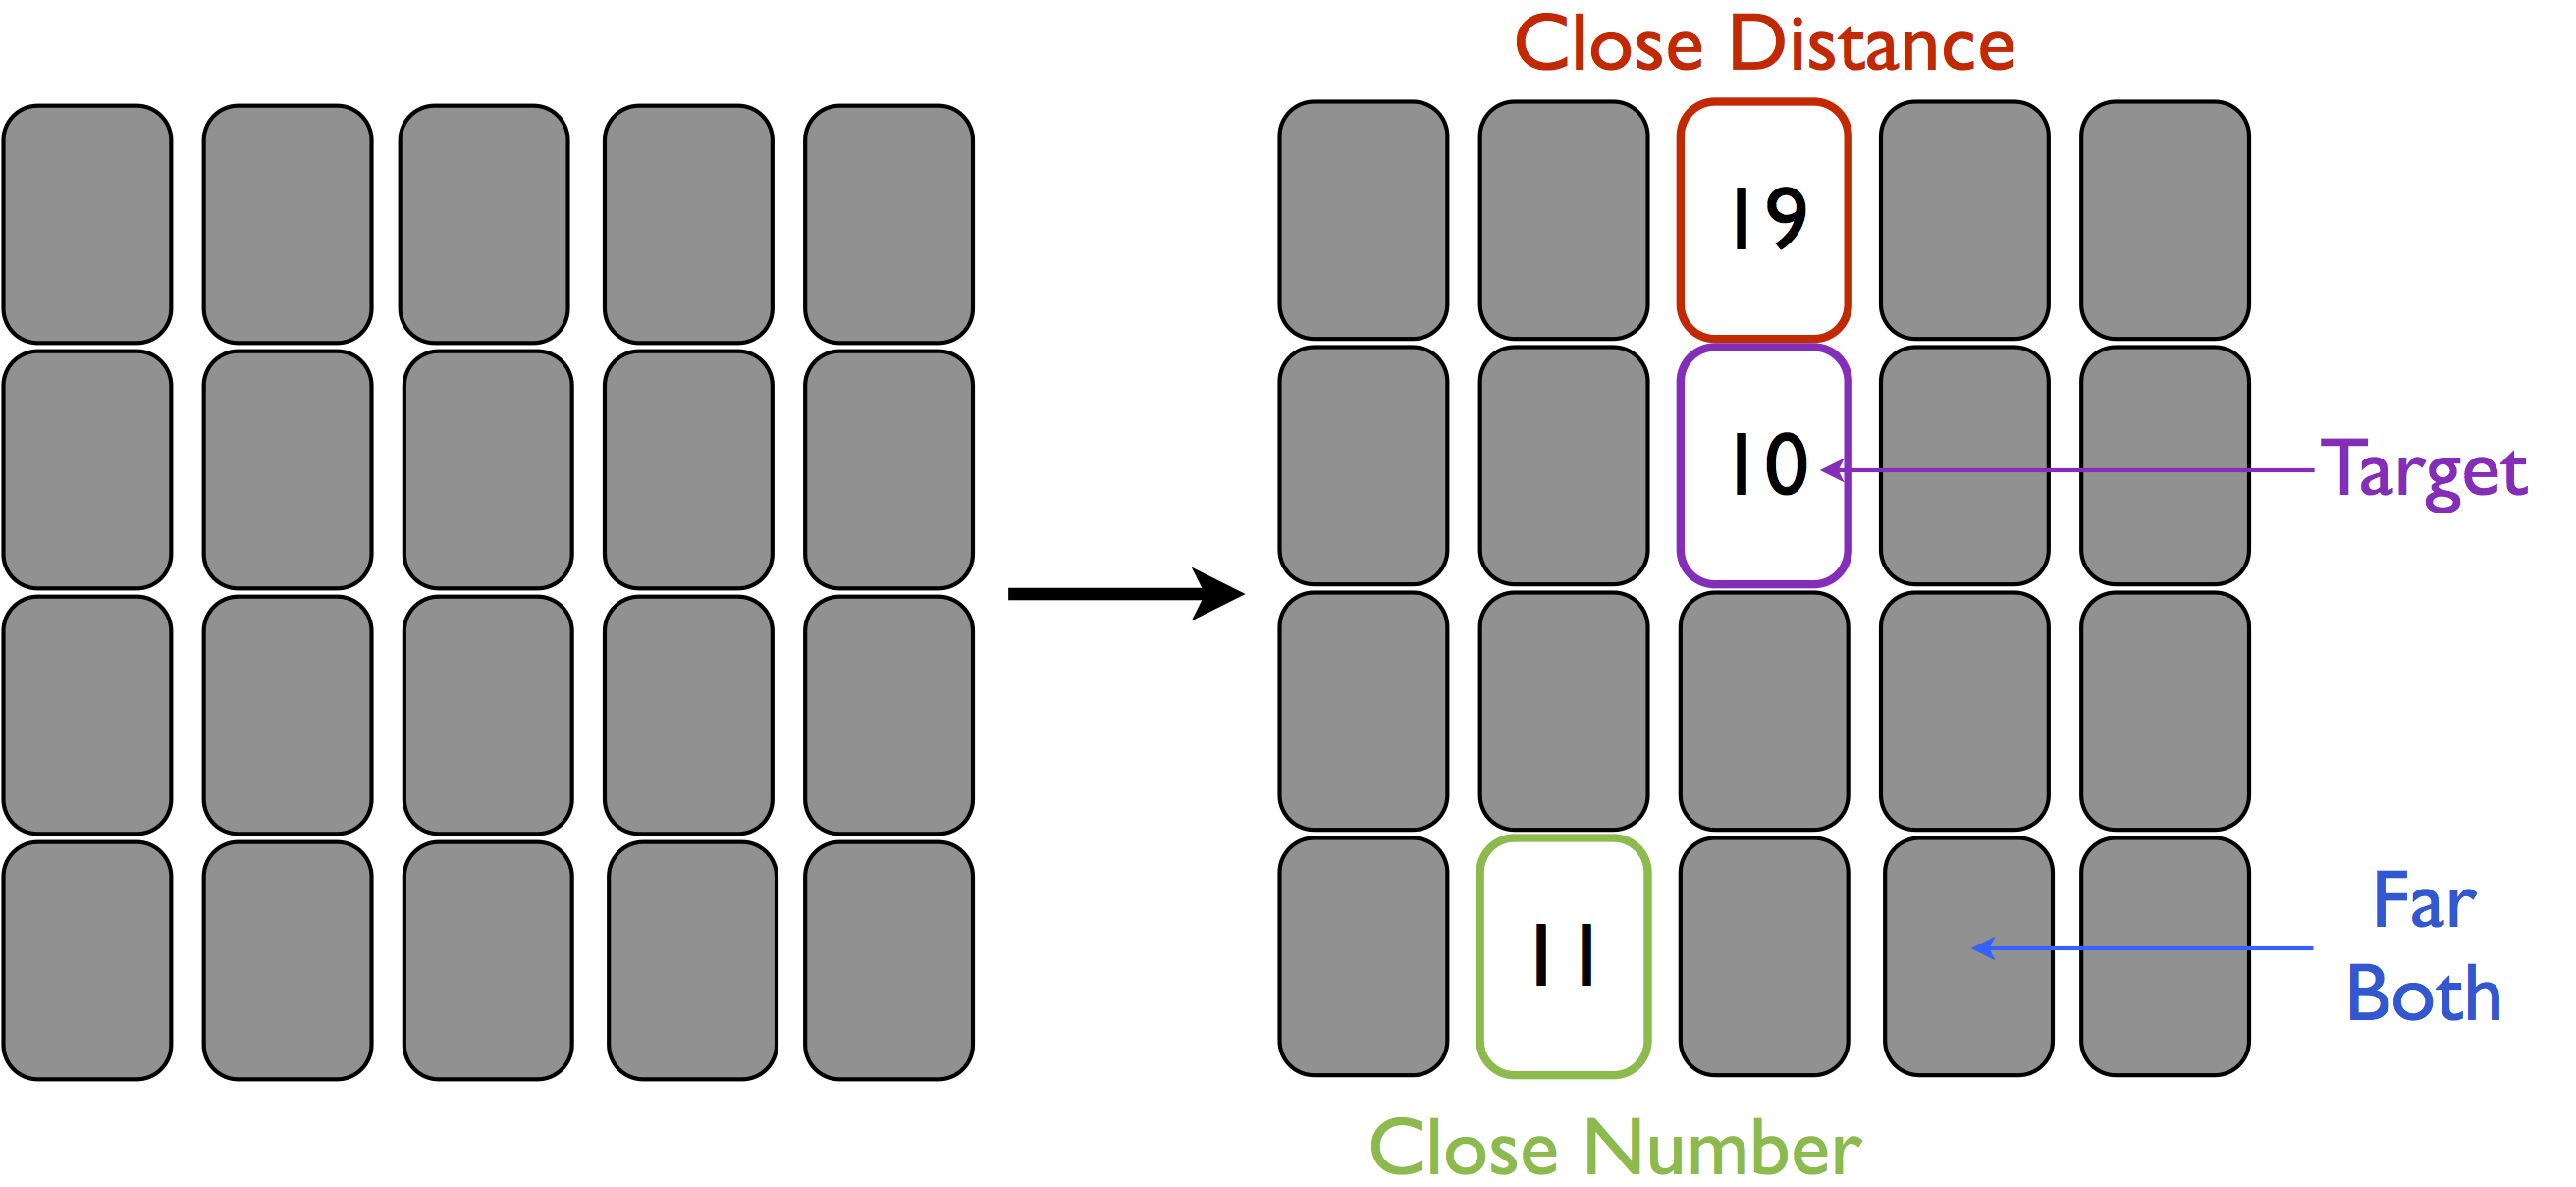
\includegraphics[width=\columnwidth]{images/card_paradigm.png}
\caption{ Expt 2 Paradigm, \textit{Position} condition. Characters' goal is to pick the card with 10 on it. In the ``Close Distance vs. Close Number" trial, one character picks the card with 19 on it, outlined in red (\textbf{Close} in physical \textbf{Distance}, far in number), and another character picks the card with 11 on it, outlined in green (\textbf{Close} in \textbf{Number}, far in physical distance). The target card is then revealed, outlined in purple. In other trials, one of the characters picks 1 (indicated in blue; \textbf{Far} in \textbf{Both} physical distance and number). }
\label{Expt2ParadigmFig}
\end{figure}


	For comparison, we included two other trials with a character who was far on both distance and numerosity. In the ``Close Distance vs. Far Both" comparison, participants saw Scott (who picked the 19 card) and David, who picked a card with 1 on it, which is far along both physical distance and numerosity. In this case, David's card is 9 numbers away from the winning card, which is the same numerical distance as Scott's card. In the ``Close Number vs. Far Both" comparison, participants saw Frank (who picked the 11 card) and David. In this case, David's card is just as far in physical distance from the winning card as Frank's card.


	In the Choose-\textit{Number} condition, participants were presented with a game with slightly different rules. There were the same 20 cards, and a target card (circled in purple), all face-down. Characters had to guess the number behind the target card. After picking a number, the card with the picked number was revealed. The characters were the same as in the \textit{Position} condition, i.e., on ``Close Distance vs. Close Number" trials, Scott picked the number 19 (\textbf{Close distance}) and Frank picked 11 (\textbf{Close Number}). After the character made their guesses, the winning number behind the target card is revealed to be 10. Similar to the \textit{Position} condition, the \textbf{close distance} character's card was close in physical distance, but far in numerical distance; whereas the \textbf{close number} character's card was close in numerical distance, but far in physical distance. Participants then attributed emotions to the two characters, and made a forced-choice judgment about who felt worse. There were similar ``Close Distance vs. Far Both" and ``Close Number vs. Far Both" trials.


\begin{table}
\scalebox{0.7}{
\begin{tabular}{l|c|c}
Near-Miss & Illusory control over \textit{Position} & Illusory control over \textit{Number} \\
\hline
\textbf{Close Distance} & \multirow{2}{*}{\checkmark \checkmark} & \multirow{2}{*}{\checkmark}\\
far number & & \\
\hline
\textbf{Close Number} & \multirow{2}{*}{\checkmark} & \multirow{2}{*}{\checkmark \checkmark} \\
far distance & & \\
\hline
\textbf{Far both} & \multirow{2}{*}{-}  & \multirow{2}{*}{-} \\
(distance, number) & &
\end{tabular}
}
\caption{Predictions for Experiment 2. Near-miss effects are predicted to be strongest when agents are close on dimensions over which they have illusory control.}
\label{Expt2Predictions}
\end{table}


\subsubsection{Predictions.}
	To reiterate, in the \textit{Position} condition, the number of the goal was known (10) whereas the position was unknown -- characters picked a position and were assigned a number (based on their choice). In the \textit{Number} condition, the position of the goal was known, but the number was unknown -- characters picked a number and were assigned a position. The two conditions differed in which dimension (position or number) the characters had control over. Importantly, the games were still random events, and the agents' control is merely illusory. For example, consider the \textit{Position} condition. One can imagine a possible counterfactual statement generated by Scott, the close distance character: ``if only I had chosen the card one position down". However, if the games were truly random, his re-picking a different card position would still have given him the same 1/20 chance of winning.

	Our predictions are summarized in Table \ref{Expt2Predictions}. In the \textit{Position} condition, the characters chose the physical position of a card, and we predicted that near-misses along physical closeness would be weighted more than near-misses along numerical closeness. In other words, the close distance character would be judged to feel the worst, then the close number character, then the far character. On the other hand, in the \textit{Number} condition, the characters chose the number, and so we predicted that near-misses along numerical closeness would be weighted more than near-misses along physical closeness: the close number character would be judged to feel the worst, then the close distance character, then the far character.


\subsubsection{Results.} Nine participants were excluded for failing the attention checks. When we examined individual emotion ratings, none of the comparisons in the \textit{Position} condition came out significant. For the \textit{Number} condition, as compared to the far character, the close number character was judged to feel more disappointed ($t(43)=2.81, p=.007$), more regret ($t(43)=2.44, p=.02$), more sadness ($t(43)=2.54, p=.015$) and less relief ($t(43)=2.12, p=.04$). For closeness judgments, in the \textit{Position} condition, both the close distance and close number characters were judged to be closer to winning than the far both character ($t(20)=3.5, p=.002; t(41)=4.1, p<.001$ respectively), and in the \textit{Number} condition, the close number character was judged to be closer than the close distance ($t(22)=4.4, p<.001$) and the far both characters ($t(43)=8.2, p<.0001$).



\begin{figure}[htb!]
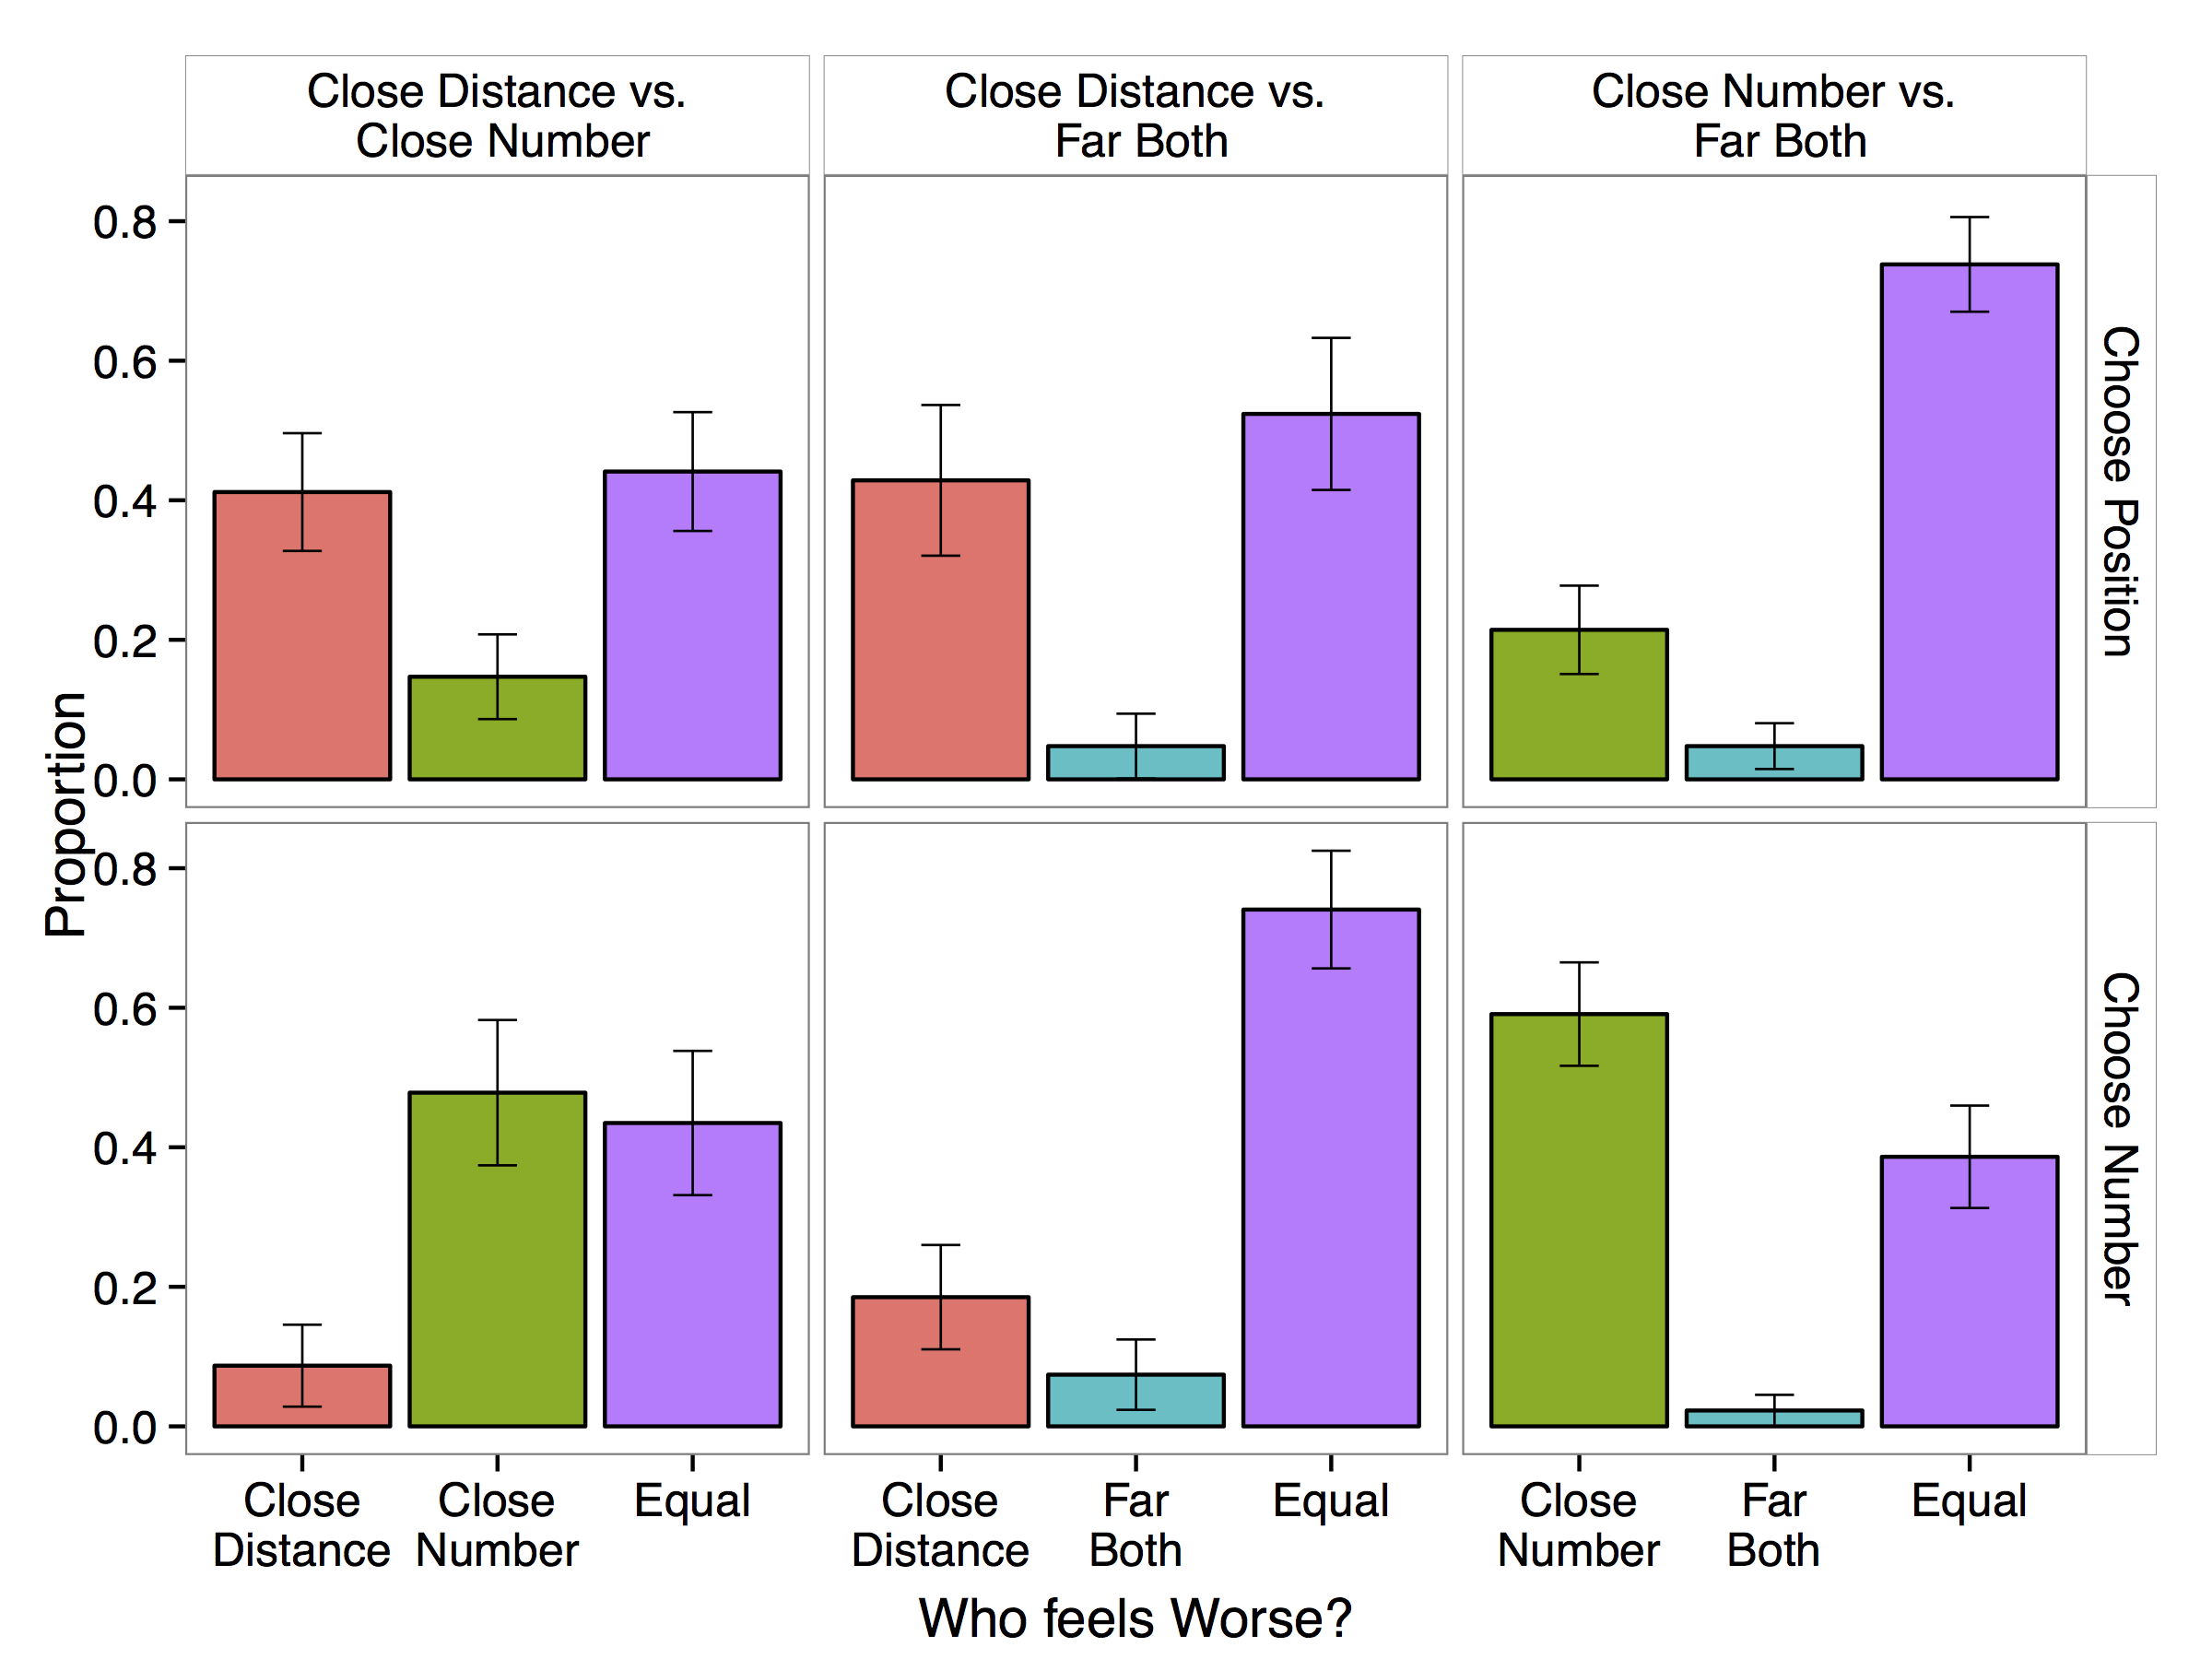
\includegraphics[width=\columnwidth]{images/cardCombined_forcedWorse.png}
\caption{ Expt 2 Results. Proportions of forced choice response. Error bars indicate standard errors. Top row: Choose \textit{Position} condition. Bottom row: Choose \textit{Number} condition.}
\label{Expt2ResultFig}
\end{figure}


The results for the forced-choice ratings are in Fig. \ref{Expt2ResultFig}. In line with our predictions, in the \textit{Position} condition, the close distance character was judged to feel worse than the close number (bootstrap, 10,000 iterations, $p=.023$) and the far characters ($p=.003$). To a smaller extent, the close number character was judged to feel worse than the far character ($p=.016$). This, together with the closeness judgment result above, suggests that participants might still be sensitive to numerical closeness even when it is task-irrelevant, perhaps because comparing numerical differences is often important in daily life. By contrast, we see the opposite pattern in the \textit{Number} attributions: The close number character was judged to feel worse than the close distance character ($p=.002$) and the far character ($p<.0001$), and there was no difference between the close distance and far characters ($p=.17$). 


The results suggest that participants are sensitive to near-misses along multiple dimensions, in this case, both physical closeness and numerical closeness. When given multiple dimensions, participants weight the dimension on which the characters would likely feel more illusory control (physical closeness in the \textit{Position} condition and numerical closeness in the \textit{Number} condition) more than the other dimension. When characters have to pick the physical location of the card, participants attribute more near-miss effects along physical closeness, and when characters have to choose a number (rather than a location), participants attribute more near-miss effects along numerical closeness. Again, it is worth reiterating that characters only have an illusion of control along these dimensions, yet this illusion of control, much like actual control, affects participants' judgments of emotions.





%%%%



\section{Quantitative modeling via meta-analysis}
	Next, we performed a meta-analysis of three prior experiments designed to examine the features underlying affective cognition in a gambling paradigm. We explicitly model the near-miss effect in a quantitative model of affective cognition.
	
\subsubsection{Participants and procedures.}
	690 participants were recruited across 3 different experiments\footnote{https://cocolab.stanford.edu/cogsci2015/nearmiss/metaAnalysis/} previously reported in \citeA{OngAffCog}. The trial involved watching a character spin a wheel and win the amount the wheel landed on (Fig. \ref{Expt3ParadigmFig}). Participants then attributed 8 emotions (\textit{happy}, \textit{sad}, \textit{anger}, \textit{surprise}, \textit{disgust}, \textit{fear}, \textit{content} and \textit{disappointment}) to the character after the outcome, using 9 point Likert scales. Each participant saw 10 trials, and the payoff and probability structure of the wheels were varied systematically to decorrelate the amount won with the expected value of the wheel. The first experiment only had these wheel trials: the second and third had wheel trials intermixed with emotion attribution trials given other stimuli (faces and utterances) instead of wheels. We took the subset of wheel trials from the second and third experiment, and the whole first experiment, to amass a dataset of 3048 observations from 690 participants.
	
	These experiments were designed to test how different features of the situation, namely the amount won and the prediction error (the amount won relative to the expected value of the gamble), affected observers' attribution of emotion to the character. Yet, because we randomized the position on which the spinner lands, these experiments incidentally provided a valuable dataset to test for near-miss effects.

\begin{figure}[htb!]
\begin{center}
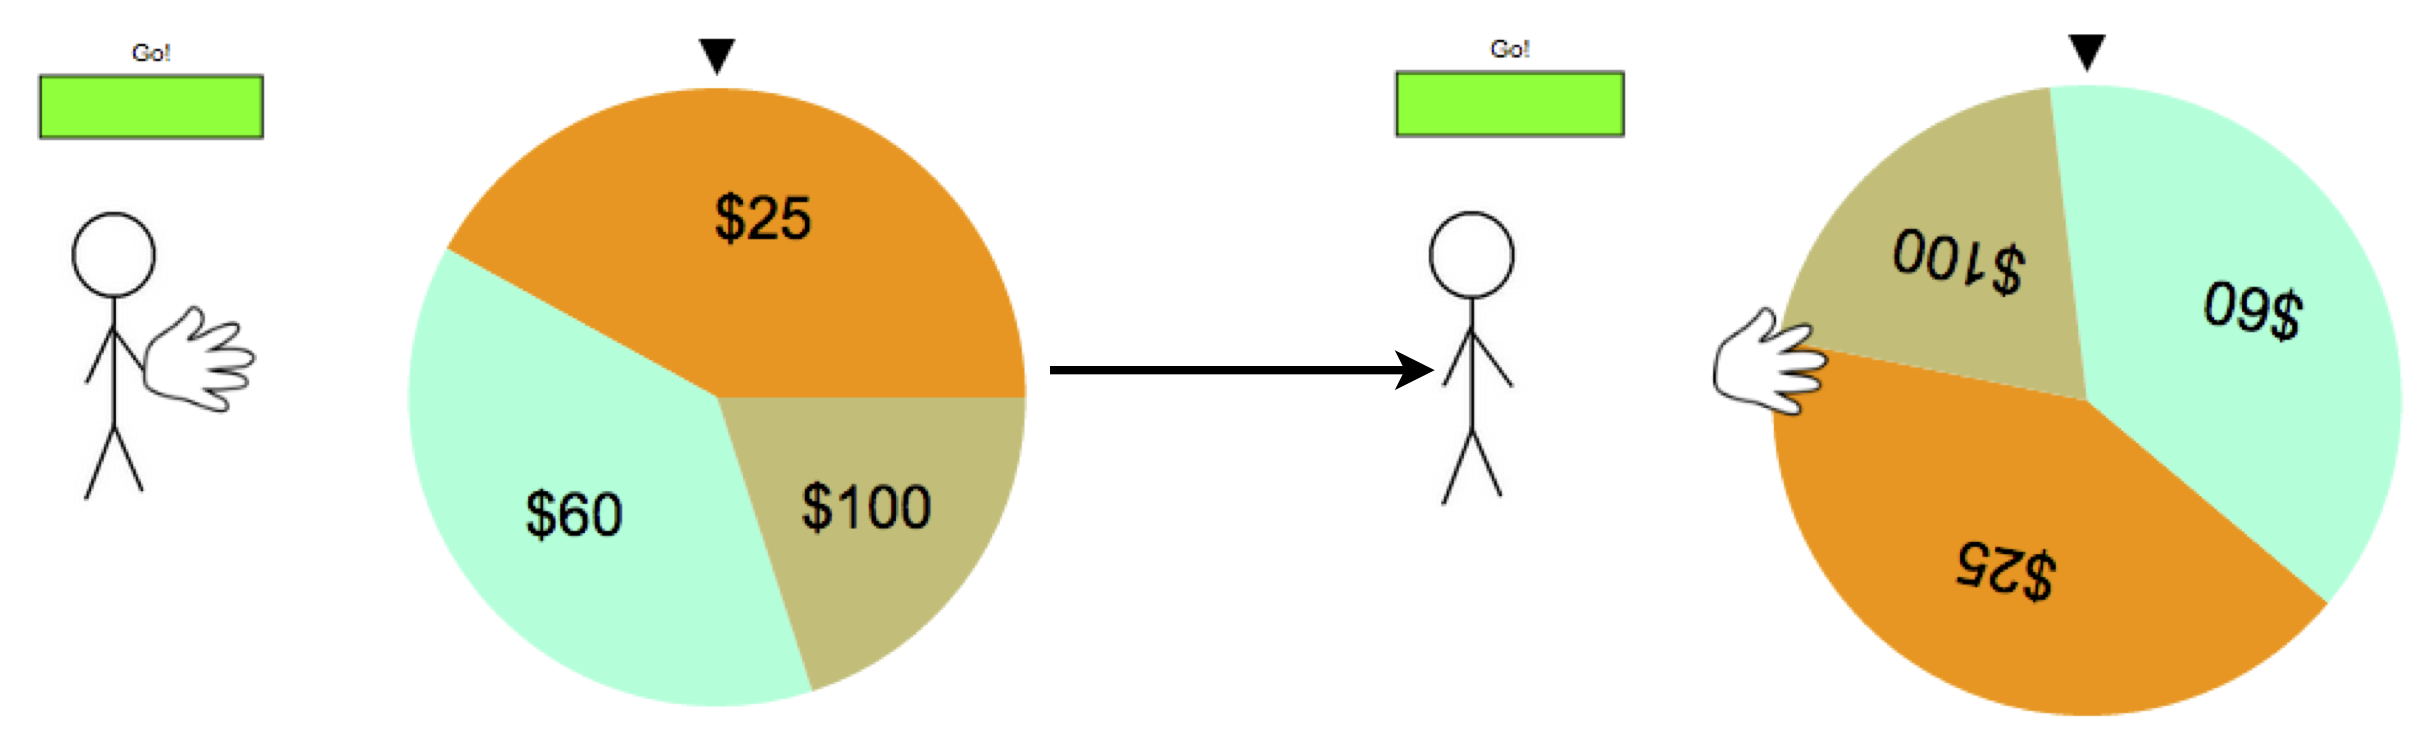
\includegraphics[width=.85\columnwidth]{images/expt3Paradigm.png}
\end{center}
\caption{ Paradigm for the meta-analysis. Participants attribute emotions to an agent after the outcome of a spin. After this spin (right), the agent won \$60 (as indicated by the black pointer), but almost won a higher amount of \$100. }
\label{Expt3ParadigmFig}
\end{figure}


\subsubsection{Previous model.} The model in \citeA{OngAffCog} incorporated three important features: the amount won (\textit{win}), the prediction error (\textit{PE}), and the absolute value of PE (\textit{absPE}). The emotion E attributed to the agent after event X was:
\begin{align}
E(X) &= b_0 + b_1 \text{win}(X) + b_2 \text{PE}(X) + b_3 \text{absPE}(X) + \epsilon \label{PEModel},
\end{align}
a linear combination of \textit{win}, \textit{PE} and \textit{absPE}. The absolute value of the PE was added to test for nonlinearities, namely, loss aversion, whereby agents will be more sensitive to negative PE values and weigh them more than positive PE values. Separate models were fit for each emotion. More discussion can be found in the paper. Eqn. \ref{PEModel} provided the starting point for the model in the following analysis.


\subsubsection{Adding Near-Miss to the model.}

Next, we proceeded to define a near-miss distance. We calculated a normalized ``distance from the edge" which ranged from 0 to 0.5, with 0 being the boundary edge between the current and closest sector and 0.5 indicating the exact center of the current sector. We then took a reciprocal transform ($1/x$) to introduce a non-linearity that favors smaller distances. Finally, we multiplied the transformed distance with the difference in payment amounts from the current sector to the closest sector. This last component was to account for the difference in utility in the two payoffs. Hence, the near-miss term we defined was:
\begin{align}
NM(X) &= \frac{1}{\text{distanceToEdge}(X)} * \Delta\text{Payoffs}(X) \label{NMRegressor}
\end{align}
which we added to the model in Eqn. \ref{PEModel}. To illustrate, for the result shown in Fig. \ref{Expt3ParadigmFig}, the distance is .05 (5\% of the sector size away from the \$60-\$100 boundary), and the $\Delta$Payoff is 60-100 = -40, as \$100 is the next nearest sector.

\subsubsection{Meta analysis results.}

We fit a linear mixed-effects model with the amount won, PE, absPE, and the Near-Miss (NM) term (Eqn. \ref{PEModel}, \ref{NMRegressor}) as fixed effects, and random intercepts by participant, wheel, and experiment. There is a significant slope on the NM term ($b = \text{-}3.5 * 10^{\text{-}5}, t(682)=\text{-}2.80, p=0.005$) on happiness. There was no significant differences between NM terms when the next-nearer outcome was positive or negative ($\chi^2(2)=0.13, p=0.94$). To understand the magnitude of the NM term, consider the slopes on win ($b = 0.0405, t(682) = 7.08, p<.0001$), PE ($b=0.036, t(682)=5.86, p<.0001$), and absPE ($b=\text{-}0.015, t(682) = \text{-}2.83, p=.005$), and the example in Figure \ref{Expt3ParadigmFig}. Not considering the near-miss effect and all else being equal, if the result had changed from \$60 to \$100, there will be an \textit{increase} in happiness due to win, PE and absPE of $40*(.0405+0.036+(\text{-}0.015)) = 2.46$ points on a 9 point Likert scale. By contrast, if we moved from the center of the \$60 sector to a distance of .01 (1\% of the sector size) away from the \$60/\$100 boundary, there would be a \textit{decrease} in happiness of $40*(1/0.5 - 1/0.01)*(\text{-}3.5 * 10^{\text{-}5}) = 0.137$ points on a 9 point scale. Thus, in this gambling scenario, the effect of a near-miss on subjective happiness attributed is on the order of 5\% of the relative happiness of winning the next higher amount. Getting a near-miss on the \$60 wheel in Fig. \ref{Expt3ParadigmFig} and narrowly missing the \$100 sector (narrowly missing winning \$40 more) has a subjective cost equivalent to losing about \$2, compared with a far-miss (landing in the center of the sector). 

This is a small effect relative to actually winning, yet it is a large and not insignificant effect considering that it does not depend on changing actual payoffs, but relative closeness. 

%%NDG: this sentence was dross to me, but you can add it back if you want.
%Consider too, that this is a stylized game of chance, with fictional characters and hypothetical gambles, which all might lead to underestimating the size of the true effect in real-life situations like missing planes.

%\red{NDG: i like this result. clear, understandable, and contextualized. it may be that we'll want to include it in our psych rev revisions...}

\section{Discussion}

Near-misses matter emotionally; here we produce novel insights about how observers' incorporate near misses into their lay theories of emotion. First, people incorporate near-misses in situations even in random situations under which agents have no direct control over outcomes. Second, this effect might reflect observers' tendency to imbue agents with \textit{illusory control} over even demonstrably random outcomes.  Consistent with this idea, observers factored near-misses more heavily into their emotion attributions when near-misses occurred within a dimension (e.g., location or number) over which agents made a choice on, even though agents could not \textit{actually} control their ability to win or lose based on their choice. Third, using a meta-analysis of three previous experiments, we modeled near-misses and compared their effect size to emotions associated with actual wins and losses. Crucially, this allowed near-misses to be incorporated, for the first time, into a quantitative model of affective cognition.

	Many open questions concerning near miss effects remain. For instance, how does a near-miss compare with its positive counterpart, the relatively-less-studied ``just-hit" (when an agent narrowly wins by a small margin)? Although there are some qualitative differences between near-misses and just-hits (e.g., the frequency of downward and upward comparison, \citeNP{Roese1997, Sweeny2012}), our meta-analysis revealed no difference between positive and negative close comparisons (near-miss and just-hits).  This suggests that outcome closeness works similarly in positive and negative domains, but future work should investigate this further.

	Our results suggest some interesting properties about near-miss judgments in scenarios where the outcome is randomly-generated. Future work will have to unify this and previous, more general work on counterfactual judgments into quantitative models of affective cognition. The model in our meta-analysis already had consideration of counterfactual judgment with its prediction error terms, yet it still does not capture the complete story. For example, related work in counterfactuals more generally has shown that the temporal recency of the counterfactual event \cite{Miller1990}, and whether the outcome resulted from an act of omission or an act of commission \cite{Kahneman1982, Landman1987} both affect judgments of emotion. How might these features of counterfactuals interact with near-misses and fit into a computational model of affective cognition? 


	Third, it is interesting to consider whether or not near miss effects in observers' theory of emotion are rational.  On its face, ascribing more negative emotion to an agent who rolls a 5, as compared to a 1 (given the goal of rolling a 6), on a die appears demonstrably irrational, as both outcomes are random and neither is ``closer," strictly speaking, to the desired outcome. However, agents likely \textit{do} feel closer after rolling a 5, rather than a 1, \textit{do} ascribe illusory control to themselves, and hence do feel more negatively following near-, versus far-misses over random outcomes. Thus, observers' use of near misses are actually functional in helping observers understand agents' experiences.  This suggests that the near miss effects that we observed could reflect some combination of two sources: (i) observer�s own inaccurate belief that agents control random outcomes, or (ii) their accurate understanding that agents react emotionally as though they controlled those outcomes.  Further work should unpack this question.

	Emotion and reason are often treated separately, and contrasted. Yet emotion can be reasonable and reason can be applied to emotion, as exemplified by work on appraisal theories of emotion (\citeNP<see>{Scherer2001}). By exploring the effects of near-misses on emotion attribution in random situations we have exposed a fascinating twilight area of the mind, where observers make reasoned judgments about the less rational emotional reactions of others.   

\section{Acknowledgments}

This work was supported in part by an A*STAR National Science Scholarship to DCO and by a James S. McDonnell Foundation Scholar Award and ONR grant N00014-13-1-0788 to NDG.


\bibliographystyle{apacite}

\setlength{\bibleftmargin}{.125in}
\setlength{\bibindent}{-\bibleftmargin}

\bibliography{nearMiss_cogsci}


%% -- start older version of discussion
%Near-misses matter emotionally, and here we sought to understand how people factor near-misses into lay theories of emotion. First, we showed that people incorporate near-misses in situations even when agents have no direct control over outcomes. Second, this effect might reflect observers' tendency to attribute to agents \textit{illusory control} over even demonstrably random outcomes.  Consistent with this idea, observers factored near-misses more heavily into their emotion attributions when agents experienced near-misses over a dimension (e.g., location or number) that they made a choice on, even when agents could not \textit{actually} control their ability to win or lose at a game. Third, using a meta-analysis of three previous experiments, we quantitatively modeled the near-miss effect and compared its effect size to emotions associated with actual wins and losses. Crucially, this allowed near-misses to be incorporated into more complete models of affective cognition in ways that go beyond prior work in this domain.
	
%	As mentioned above, though near-miss effects and the broader class of counterfactual effects on emotion seem to be so intuitive, especially to the scientists studying them, there still remains many open questions. How does a near-miss compare with its positive counterpart, the relatively-less-studied ``just-hit" (when an agent narrowly wins by a small margin)? Although there are some qualitative differences between near-misses and just-hits (such as the frequency of downward and upward counterfactual generation, \citeNP<e.g.>{Roese1997, Sweeny2012}), more work has to be done to study just-hits in a similarly quantitative manner. The model in our meta-analysis takes just-hits into account with the $\Delta$Payoff term, and we found no difference between positive and negative close comparisons (near-miss and just-hits), suggesting a lack of differences; however, more in depth work should be done to investigate this further.


%
%Incorporating near-miss effects into emotion judgments, even for random events, likely makes observers more accurate:
%People \textit{do} ascribe illusory control to themselves and hence \textit{do} feel more negative affect in near-miss scenarios with random outcomes. 
%This leaves open the question of what human observers know of agents' control in these situations---do \emph{observers} suffer the illusion of (the agents') control, or do they attribute the illusion of control only to the \emph{agents}?		
%%	Thus, in order to draw accurate inferences, observers have two options. One, observers would have to ascribe illusory control over the outcomes to these agents. Alternatively, observers may understand that agents do not have real control over their outcomes, yet simultaneously recognize that agents do feel illusory control, and therefore observers account for this and attribute near-miss effects. 
%%Thus, a third line of future research should investigate the accuracy of observers' lay theories with respect to how agents actually react and feel. 
%This suggests future research into the ``lay theory of illusory control'' and how it interacts with the lay theory of emotion.

%Emotion and reason are often treated separately, and contrasted. Yet emotion can be reasonable and reason can be applied to emotion.
%By exploring the effects of near-misses on emotion attribution in random situations, we have exposed a fascinating twilight area of the mind, where rational judgments are made about less rational emotional behavior.   

%Finally, we hope that future work in social cognition and affective cognition would continue to marry both qualitative work and quantitative models, which we feel is needed to drive science forward to the next level (which we wouldn't want to nearly-miss).
	
%	Finally, it is worth considering our results in the light of bounded rationality. That is, given the ``irrational" beliefs ascribed by illusory control (that people have control over random outcomes), our results are explained by the controllability account we started with. It is interesting to consider too that if agents \textit{do} experience these near-miss effects in random scenarios, then observers incorporating these effects into lay theories are accurately drawing inferences about the agents.
	
%	It is our hope that combining qualitative studies of cognitive phenomena in judgments of emotion (to study boundary conditions) with quantitative modeling using computational models would spur progress in the overlap between the fields of cognitive and affective science, and generate theories with predictive power and application to daily life.

%% -- end old disc 

% --- start original myIntro: ---
%	When Rob achieves a desired outcome, such as winning a soccer match, we intuitively know that he would feel positive. Conversely, when Rob loses, or otherwise fails to achieve an outcome, we can reason that he would feel negative. Such intuitive reasoning about emotions comprises \textit{affective cognition} \cite{OngAffCog}, and forms an integral part of our social lives. Our intuitive theories of emotion, however, are more complex than considering just simple winning and losing: If Rob just fails to achieve the outcome by a small margin---a \textit{near-miss}---such as losing a soccer game by a single goal, we intuitively recognize that he actually would feel worse than if he had missed by a larger margin, because the outcome was ``so close" to winning. Penalty shootouts in soccer provides the most exaggerated of such near-miss scenarios: the losing team often loses because of one missed ball, sometimes an inch shy of escaping the goalkeeper's hands. These details add much more emotional intensity to all agents involved, more so than just a simple loss. Contrary to the above idiom, close \textit{does} count---\textit{emotionally}.
	
%	Psychologists have long known that near-misses form an integral, but surprisingly not well understood part of affective cognition, or reasoning about emotions \cite{Johnson1986, Gleicher1990, Teigen1996}. Most of this work falls under the broader category of counterfactual thinking, or thinking about ``what might have been" \cite{Bryne2002,McMullen2002, Medvec1997, Roese1997}. Near-miss counterfactuals are particularly engaging, because these possible worlds almost happened: they were separated from the current world by some small ``distance". Consider \citeA{Kahneman1982}'s classic example of Mr Tees, who missed his plane by 5 minutes, and Mr Crane, who missed his plane by 30 minutes. People consistently judge the person who narrowly missed his plane to feel much worse than the one who missed it by a wider margin.
	
	

%	There however, remains many open questions regarding the nature of the near-miss effect in observers' lay theories of emotion. First, why does the near-miss effect hurt? One explanation is that agents (the targets of observers' reasoning) experiencing a near-miss could have done something different to achieve the desired outcome, increasing feelings of regret \cite<e.g.,>{Zeelenberg1998}. For example, Mr Tees could have left his home slightly earlier, and might have caught his plane then. Agents can exercise control over the situation, and thus could have affected the outcome. Indeed, previous work has shown, for example, that the controllability of (non-near-miss) outcomes affects counterfactual thinking (whether upward or downward counterfactuals are generated) \cite{Roese1995}. If near-misses are judged to hurt because of an agent's potential to have changed the outcome via a different action, then observers should only attribute near-misses to agents in situations where agents have control. This account should then predict that observers should not attribute near-miss effects when the outcome is outside the agent's control, such as in games of chance or other random events. That is, observers should not rate agents as feeling worse if the agents miss a demonstrably random goal by a small, compared to large, distance. Anecdotally, however, one might be able to think of people who narrowly missed winning a prize in a raffle, lottery, or lucky draw, as feeling bad because they ``just missed" winning. Previous work has also shown that gamblers showing increased motivation and persisting in gambling more after near misses, even though the outcome of games like slots are independent of the gambler's actions \cite{Kassinove2001, Reid1986}. In Experiment 1, we sought to test this further by examining whether observers incorporate near-misses in their judgments of others' emotions even in random scenarios. We show that observers readily judge an agent who ``narrowly misses" on a die game (by rolling a number close to the target number) to feel worse than one who misses by a larger amount, even though outcomes on a die game are not ordered like the number line.

%	Second, when presented with multiple possible types of distances in random situations, how do observers weight these types of distances in their affective judgments? In any particular situation, there could be more than one \textit{dimension} of closeness. For example, if Rob narrowly loses a soccer game by one goal, one might consider distance along physical space (how physically close his goal attempts came to scoring), or along time (if the goal against his team came in the last few minutes of the game), just to name several dimensions. If we return to our discussion on games of chance, however, there could be several such dimensions as well, all of which are still out of the agent's control. One hypothesis is that observers might judge agents to feel some sort of ``illusory" control over games of luck (like the ``hot hand fallacy" or ``gambler's fallacy" that people use in judgments of winning probability, e.g., \citeNP{Roney2009}), and hence incorporate near-misses along those dimensions. Given multiple dimensions, this hypothesis would predict that observers would weight dimensions along which the agent has more illusory control over other dimensions. To illustrate this concretely, imagine that one was flipping over numbered cards trying to match a given target number. In this case, the agent has control over the position of the picked card, even though the number on the back of the card was out of his control. If he loses, there are thus two distances at play: the physical distance of the picked card to the target card, and the ``numerical distance" from the picked card to the target card. Our prediction would be that because the agent has control over the physical position of the picked card, observers would weight near-misses along physical proximity more than near-misses along numerical closeness. By contrast, if the game was slightly changed to be guessing the number behind a target card, and after the agent picks a number, the card holding the picked number was revealed. In this case, the agent has control over the number, and so we predict that observers would weight near-misses along numerical closeness more than along physical closeness. One might argue that physical closeness in the latter game is irrelevant, but so is numerical closeness in the former game. In fact, if the games were truly random, both dimensions in both versions of the game are out of the agent's control\footnote{In the former version where the agent picks the position of a card, and if the agent picks the card next to the winning card, one can imagine the agent generating the counterfactual ``oh if only I had picked the neighboring card". However, if the cards were truly randomly dealt and the agent repicked the neighboring card, he would still have had the same uniform chance of winning. One can consider an analogy to re-rolling a dice; the outcome is still randomly-generated.}. In Experiment 2, we directly test this hypothesis of illusory control, and show that observers incorporate larger near-miss effects along dimensions that the agent has illusory control over.

%	Finally, how much does a near-miss cost psychologically? That is, what is the size of the near miss effect (narrowly missing a desired outcome) relative to the happiness of actually obtaining said desired outcome? In Experiment 3, we build upon a previous model of affective cognition \cite{OngAffCog}. This model used a gambling paradigm that allowed us to parametrically vary features of the situation that affects judgment of emotions, such as the payoff structure and the distance to the neighboring outcomes. We explicitly incorporate modeling of near-miss effects into this existing quantitative model, which allowed estimates of the relative effect sizes and a better quantitative understanding of near miss judgments. More importantly, this enables the integration of near miss emotional judgments into existing models of affective cognition, and allows the construction of more comprehensive models of affective cognition.  

%	In summary, this paper makes three contributions: we explored (i) whether people incorporate near-misses in their intuitive theories of emotion for scenarios with randomly-determined outcomes; (ii) whether people might do so because of the illusion of control over these outcomes; and (iii) how much near-misses cost relative to winning and losing, via incorporation of near-misses into a quantitative model of affective cognition.
% ---end original myIntro ---

%Near-misses matter emotionally, and in this paper we sought to understand how people factor near-misses into lay theories of emotion. First, we showed that people incorporate near-misses in situations where the agent has no direct control over the outcome, such as the random outcome of a die roll---such numbers are generated by chance and numerical closeness has no actual relevance to the outcome, yet people seem to infer an illusory relevance. Second, when presented with multiple dimensions of closeness, people weight near-misses more when the near-misses fall along a dimension on which agents have illusory control compared to dimensions along which agents do not have such control. Third, using a meta-analysis of three previous experiments with a gambling paradigm designed to study features of affective cognition, we were able to quantitatively model the near-miss effect. This analysis allowed a comparison of the size of the near-miss effect relative to actually winning the next alternative. Additionally, this allows near-misses to be incorporated into more complete models of affective cognition.
%-- end original myConc


%	\red{NDG: be clearer here: first, even if people are sensitive to causally-irrelevant dimensions, do they weight causally-relevant ones more? second, is this weighting flexible in the sense that it readily adjusts to contextual factors (not just e.g. physical factors)?}
%	Second, how do observers reason using these distance dimensions? In any particular situation, there could be more than one dimension of closeness, although not all of them would be causally-relevant, or otherwise relevant to the task at hand. Depending on the context, different dimensions of distance should matter to different extents. For example, if one was flipping over numbered cards trying to match a target number, is the proximal distance of the chosen card to the target card relevant? Is the numerical distance of the chosen card to the target card relevant? For the former, yes, and for the latter, much less so. What about if one was guessing a number and writing it down instead? In that case, numerical closeness should matter more. In Experiment 2, we show that observers are sensitive to contextual information (the rules of the game and the information that is presented) that changes the relevance of different distances in a random card-guessing task, and spontaneously alter their judgments during the task when presented with additional information.
%\textcolor{red}{(to discuss with Noah more on this point. action-outcome contingency.)} %not sure how to add this in.
	
	
	
	%One proposed \textit{causally-relevant} explanation for the near miss effect is that of controllability: Mr Tees could easily think of actions he could have done differently (``if only I woke up ten minutes earlier") that would have led to him catching the plane. \red{NDG: controllability isn't explained clearly here, and no alternative is given, so it isn't clear why you mention it.}


%% Can this paragraph fit here? or should it belong between the end of the Intro and the start of Expt 1, in a section called "Predictions" (that was the way I had it initially).
%	Based upon findings from previous work \cite{Kahneman1982, Johnson1986, Gleicher1990}, we can list several predicted properties of near-miss effects. See Fig. \ref{PredictionFig} for an illustration, where we have included both near-miss and just-hit effects, although we focus on the former in this paper. First, the near-miss effect should be \textit{non-linear} with respect to distance to the desired outcome---the near miss effect should only occur at small distances, and should matter increasingly more with increasingly smaller distances. Second, the magnitude of the near-miss effect should be \textit{small but proportional} to the difference between the desired and undesired outcome.
%\red{NSG: these properties are predicted from your graph, but it's not clear where your graph came from -- it sounds like you're just making them up...}
%
%\begin{figure}[htb!]
%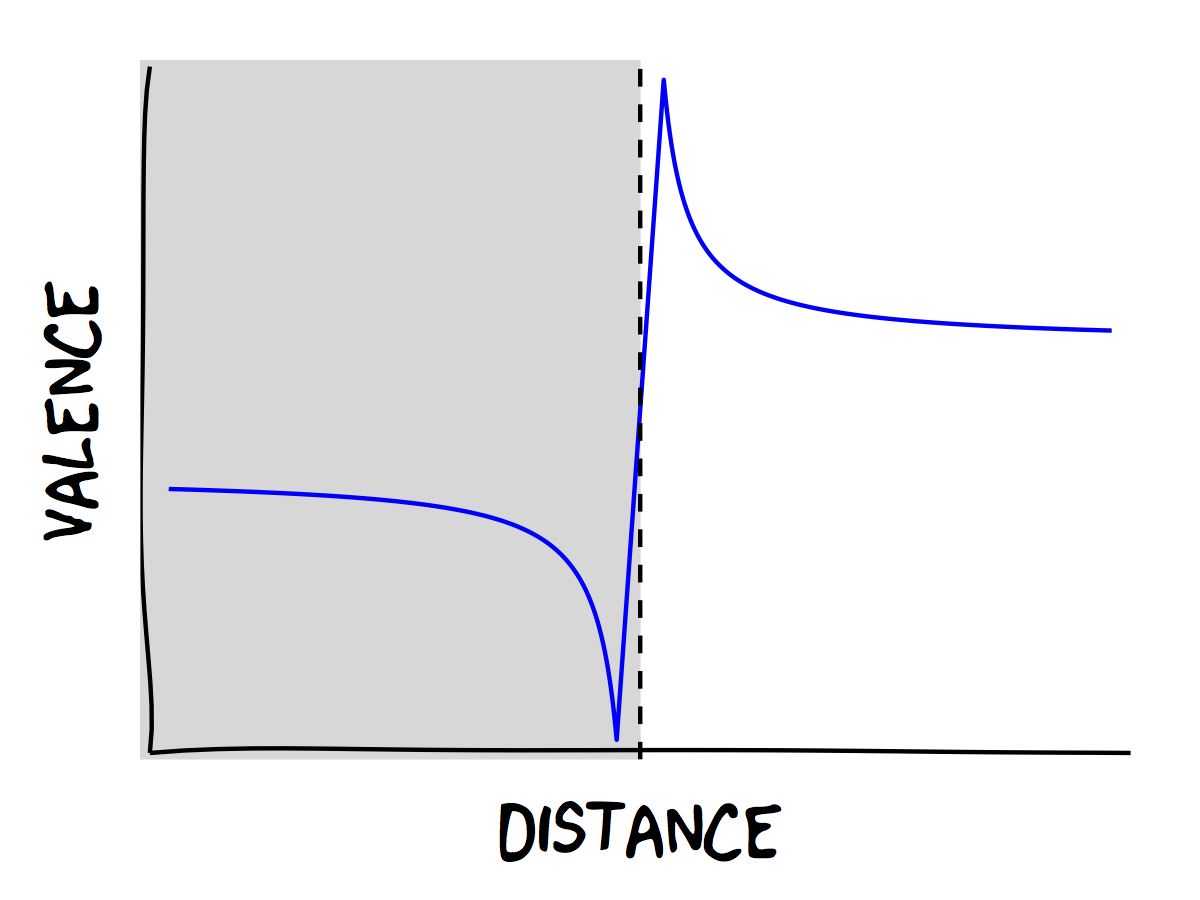
\includegraphics[width=\columnwidth]{images/predictionFig.png}
%\caption{ Prediction. A plot of emotional valence against ``distance" to the counterfactual world, where the unshaded region represents the desired outcome, and the shaded region, the ``miss" region. Near misses and ``just-hits" are predicted to be non-linear variations of valence at small distances to the miss-hit boundary.}
%\label{PredictionFig}
%\end{figure}



% be a little less vague 
%The distances that separate the desired-but-unattained counterfactual world from the current world.

% define dimensions

%	There however, remains many open questions regarding the nature of the near-miss effect, and in this paper we address three of them. First, what are the dimensions of distance that observers judge to be relevant to an agent's emotions?  The answer most commonly proposed by the current literature asserts that people should consider causally-relevant dimensions, like the amount of time one misses a plane by. This would predict that people should not exhibit near miss effects in their lay theory when considering games of chance, or random events, as the causal process that generated the outcomes are based on chance. However, previous work has shown that gamblers persist more after near misses, showing a near-miss effect on motivation even though the outcome of games like slots are independent of the gambler's actions \cite{Kassinove2001, Reid1986}. In Experiment 1, we show that observers readily judge an agent who ``narrowly misses" on a die game (by rolling a number close to the target number) to feel worse than one who misses by a larger amount, even though outcomes on a die game are not ordered like the number line. This suggests that observers may also consider causally-irrelevant dimensions

%Observers seem to consider causally-irrelevant dimensions of distance as well, when a causally-relevant dimension does not exist.






%Spell out relevant and irrelevant. Deeper theory.

%Nearness compared to actual outcome differences



%Hmm maybe not the best example: even if the 7 mins was reduced to 0, they wouldn't necessarily have won.

%	Argentina nearly won the 2014 FIFA World Cup Final, conceding the only goal of the match with barely 7 minutes left in extra time, but as the above idiom morbidly points out\footnote{Points in horseshoes are scored based on distance thrown horseshoes land from the target stake. Thrown hand grenades, in contrast, do not need to hit their target to be effective.}, close in this case, does not count. However close they were, they did not win. However, as Argentinian supporters would attest, close does matter---\textit{emotionally}.



%	Though we live in only one of many possible realizations of the world, our mental lives---and consequently, our emotional lives---are constantly spent exploring other possible worlds via counterfactual thinking \cite{Bryne2002, Gleicher1990, Johnson1986, Roese1997}. ``Near-miss" or close counterfactual comparisons in particular, are so mentally engaging because these possible worlds had almost happened. Consider \citeA{Kahneman1982}'s classic example of missing a plane by 5 minutes, as opposed to 30 minutes: people consistently and reliably judge the person who narrowly missed his plane to feel much worse than the one who missed it by a wider margin. One proposed reason is that it is much easier to generate possible counterfactual antecedents that would have resulted in the counterfactual consequent of catching the plane. The near-miss character could easily generate counterfactuals like ``If only I woke up 5 minutes earlier" or ``if only I had packed my bag the night before", that would result in the consequent ``then I would have caught my plane". If the counterfactual world is somehow \textit{closer} to the current world, then perhaps the counterfactual world would only require a smaller change in the causal chain that led up to the current world in order to be realized.
%
%	Previous research has identified some of the impact of closeness on counterfactual thought \cite{Kahneman1990, Teigen1996}. Closeness increases the activation of counterfactual thought, by increasing the salience of the counterfactual world \cite{Kahneman1982, Roese1997}, and additionally also amplifies the affective consequence of the counterfactual comparison \cite{Johnson1986, Kahneman1982}. Narrowly missing a plane or a World Cup Title feels far worse than missing it by a large margin. 
%	
%	Yet, there remains many open questions regarding the nature of these distances. What are the relevant dimensions of closeness that people incorporate into their lay theories of the world, and into their lay theories of emotion? Intuitively, people should consider only causally-relevant dimensions, like the amount of time one misses a plane by. However, anecdotally we are reminded of many instances where a (randomly-generated) lucky draw number is announced, and the holder of a (randomly-assigned) lucky draw ticket that is off by 1 number expresses extreme negative emotions. Given the random nature of this game, his number is not any ``closer" to reality than any other number in the set of possibilities.
	
	

%\subsection{Outline of paper:}
%\begin{enumerate}
%\item Lay out near miss predictions. Noticably: clearly, on both win and lose sides.
%\item Expt 1: just show it with vignettes, where distance is causally related to outcome
%\item Expt 2: show it with die vignettes, where distance is irrelevant
%\item Expt 3: card task, show that the relevant dimension can be tweaked
%\end{enumerate}
%
%
%
%\subsection{Contributions:}
%\begin{enumerate}
%\item ToE takes into account near misses -- but along what dimensions?
%\item show robustly that it considers both neg and positive misses (expt1)
%\item show that it considers irrelevant distances
%\item 
%\end{enumerate}
%
%Any similarity, causal counterfactual
%control-relevant (exploitable) causal counterfactual
%covert utility differences



%%% Expt 2 other conditions

%\red{NDG: contrary to expt 1??}
%, and Two-Step-Position (\textit{Two-Pos}; N=100).

%\red{NDG: it's hard to follow this section because the condition labels, etc are cryptic. how about ``close distance'', ``far both'', ``close number''. and ``position relevant'', ``number relevant''? or something that ties more closely to control -- here it's controllability i think, not simple relevance?}


%We predicted that in the \textit{Pos} condition, proximity would be judged to be a more relevant dimension of closeness than numerosity, and so the close distance character would be judged to feel worse than the close number character, although the close number character would, to a lesser extent, be judged to feel worse than the character who chose the far card. In the \textit{Num} condition, on the other hand, proximity is irrelevant, and so we predicted that the close number character would be judged to feel the worst, and there would be no difference between the close distance character and the far character. \red{NDG: why?? this doesn't seem to follow from any theory laid out so far in the paper.}

%The visual description that participants saw was similar to the \textit{Pos} condition. 

%\red{NDG: the Two-Pos condition is hard to follow.}
%The Two-Step-Position (\textit{Two-Pos}) condition was similar to the \textit{Pos} condition, except that after characters picked their cards but \textit{before} the winning card is revealed, participants make one set of emotion attributions and one forced-choice on who felt worse. Following this, the winning number 10 is revealed, and then participants make another set of attributions. Hence, participants in this condition made two sets of attributions, one before the location of the winning card is revealed (\textit{Two-Pos-BeforeReveal}), and once after (\textit{Two-Pos-AfterReveal}).

%\subsubsection{Predictions.}

%The \textit{Two-Pos} condition has an interesting twist. Prior to finding out the position of the winning card, position is still a more relevant dimension than numerosity because of the context, but participants do not yet know the position of the winning card, which makes it impossible to judge closeness based on proximal distance. In this attribution, observers should make judgments based on numerosity. There would also be no difference between the proximally close and the far characters, and we predicted that the numerically close character will be judged to feel the worse of them all (i.e., \textit{Two-Pos-BeforeReveal} results should be similar to \textit{Num}). However, after finding out the position of the winning card, proximal closeness becomes possible to judge, and so we should expect to see the proximally close character being judged as feeling the worst (\textit{Two-Pos-AfterReveal} results should be similar to \textit{Pos}).


%results

%For the \textit{Two-Pos-AfterReveal} attributions, the proximally-close character was judged to feel more disappointment ($t(31)=3.25, p=.003$), more regret ($t(31)=3.56, p=.001$), more sadness ($t(31)=2.76, p=.01$) and less happiness ($t(31)=2.67, p=.01$) compared to the numerically-close character. The proximally-close character was also judged to feel more disappointment ($t(33)=2.73, p=.01$), more regret ($t(33)=4.24, p=.0001$), more sadness ($t(33)=2.99, p=.005$), less happiness ($t(33)=2.49, p=.018$), and less relief ($t(33)=2.77, p=.009$) than the far character.

%For the \textit{Two-Pos-AfterReveal} judgments, we find them to be qualitatively similar, in line with our predictions: the proximally-close character was judged to feel worse than the numerically-close character ($p=.0001$) and the far character (bootstrap $p=0$ as there were no observations for the far character feeling worse). The numerically-close character was not judged, however, to feel worse than the far character ($p=.41$).

%In the \textit{Two-Pos-BeforeReveal} attributions, the numerically-close character is judged to feel worse than the proximally-close character ($p=.004$) and the far character ($p=.0001$), while there is no difference between the proximally-close and far characters ($p=.13$).

%The results suggest that observers are sensitive to multiple dimensions, in this case, both proximal closeness and numerical closeness, and are able to flexibly judge which is the dimension that is more relevant to the task. When characters have to pick the physical location of the card, participants attribute near-miss effects along proximal closeness, and when characters have to choose a number (rather than a location), participants attribute near-miss effects along numerical closeness. However, participants still judge near misses along numerical closeness (but to a much smaller extent) when numerosity is not a task-relevant dimension, supporting the results from Experiment 1. 
%In the Two-Step-Before attribution, for example, numerical closeness is irrelevant, but the position of the winning card is unknown, so perhaps participants are judging near-misses based on the only information available.

%\red{NDG: hmm. these results don't seem to add much to the previous lit, do they?}







%%%%% This is the basic vignette experiment %%%%%
%
%\section{Experiment 1: Vignettes}
%In Experiment 1, participants made attributions of emotion to characters in ``near-miss" or ``just-hit" vignettes.
%
%\subsubsection{Materials.} We generated 6 vignettes that involved a dimension of ``distance" which was relevant to the outcome. There were two characters in each vignette. For example, in the ``freeGift" vignette, participants read about Scott and Frank who were both in line for a free brand new vacuum cleaner. Scott was 2nd in line when they ran out of free gifts, while Frank was number 10 when they ran out of free gifts. The possible distances shown were drawn from the following possible values: \{-50, -10, -2, 2, 10, 50\}, where negative values indicates not making the desired outcome. The example described above had distances of -10 and -2. The other vignettes involved: 2) just missing a plane, 3) getting tickets for a concert, 4) making it to a gelato shop before closing time, 5) getting admitted to a course at the local community college and 6) running out of paint when painting a fence.
%
%\subsubsection{Participants.} We recruited 100 participants through Amazon's Mechanical Turk and paid them for completing the experiment. All experiments reported in this paper were conducted according to guidelines approved by the Institutional Review Board at Stanford University.
%
%\subsubsection{Procedures.} Participants viewed each of the six vignettes in a random order. After each vignette, they answered several attention check questions, before rating how each character in the story felt, along six emotions: \{happiness, sadness, contentment, disappointment, relief, and regret\}. After they attributed emotions to both characters, participants made a forced choice rating: which character felt happier? They were also given a neutral option: ``Both feel equally happy".
%
%
%\begin{figure}[htb!]
%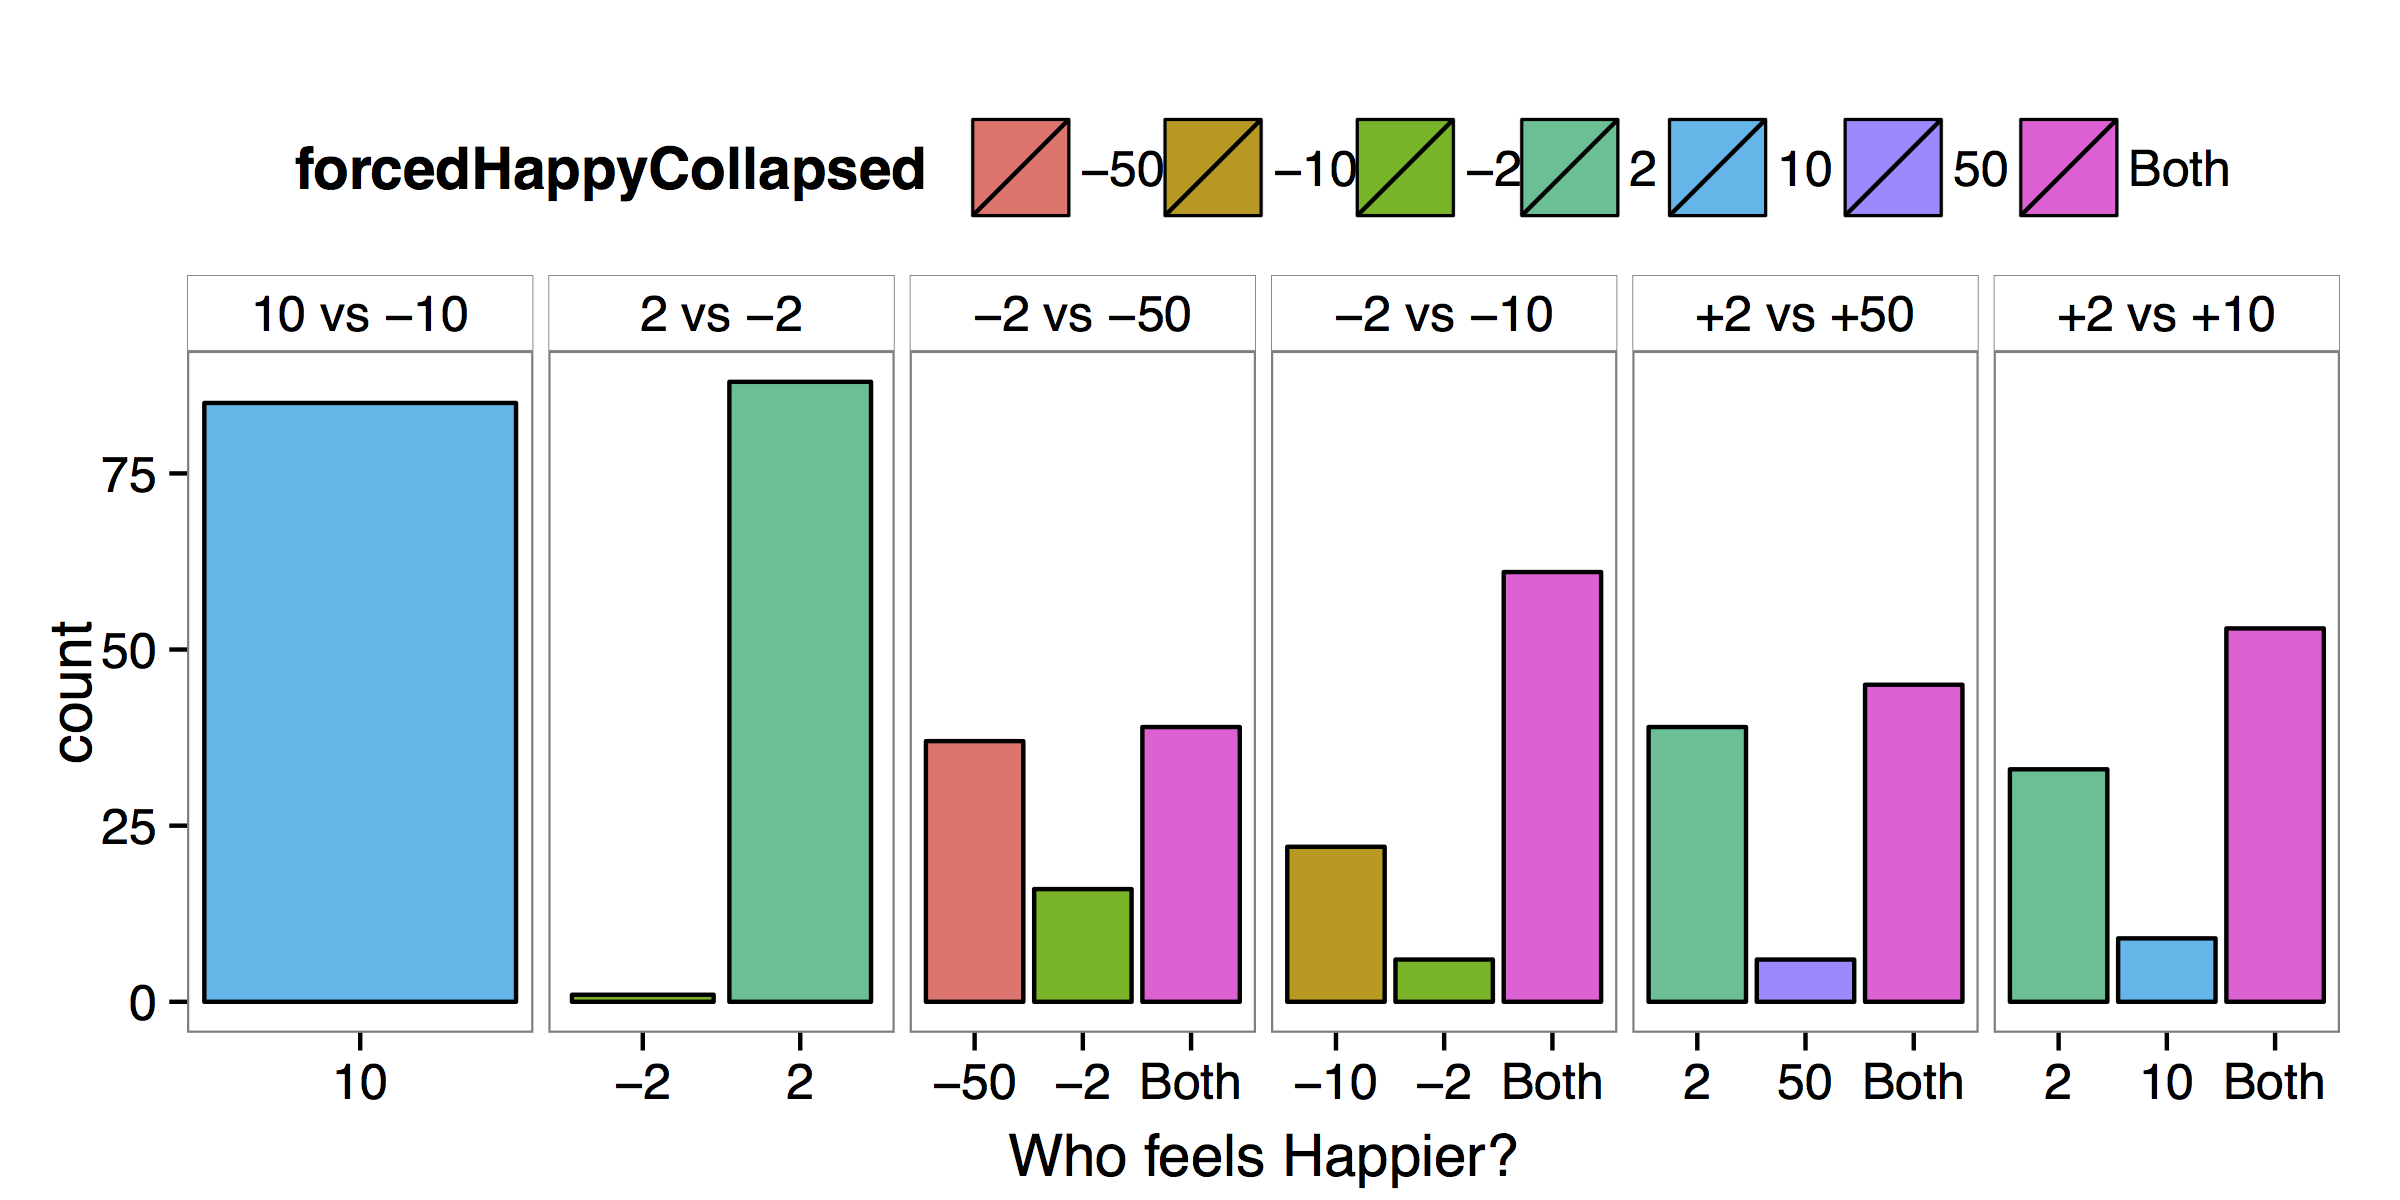
\includegraphics[width=\columnwidth]{images/vignettes_forcedHappy.png}
%\caption{ Expt 1 Results. Proportions of forced choice response to ``Who feels happier?". Error bars indicate standard errors. Answers are labeled with the distance of the character's outcome. E.g., in the right-most panel, more people judged the character who just made the outcome (+2) to be happier than the character who made it by a larger margin (+10).}
%\label{Expt1ResultFig}
%\end{figure}
%
%%%%% STATS
%
%\subsubsection{Results.} Post-hoc analysis showed that results were similar across five of the vignettes\footnote{The only anomaly was the fence painting vignette. In the critical comparison in that vignette, X ran out of paint with just 2 inches of fence left, while Y ran out with 10 inches left. Although we predicted that the near-miss character (X) would feel worse, painting a fence involves a persistent product rather than a once-off event: X could return to fence in the future, and he only needs to paint 2 more inches then. In this case, the more distance, the better. We excluded this vignette from the analyses.}: the character that experienced the near-miss (-2) was rated to feel worse than the character that experienced a further-miss (-10, -50) (STATS), and the character that just made the outcome (+2) was rated to feel better than the character that made the outcome by a large margin (+10, +50) (STATS).
%
%The forced choice results are given in Fig. \ref{Expt1ResultFig}. Across the win-lose comparison (left two panels), all participants rated the character who obtained the outcome to be happier. Across lose-lose comparisons, far fewer participants rated the near-miss character as feeling happier (STATS), and across win-win comparisons, far more participants rated the just-hit character as feeling happier (STATS). We note that a large proportion of participants chose the neutral option, and this proportion is higher than than the near-miss/just-hit judgments. 
%
%% 
%\textcolor{red}{\textit{COMMENT: do we interpret the high proportion of "Both" as meaning that it's a weak effect? or that there are individual differences, and majority of Ps might not be sensitive to this?}}
%
%
%%%%%% End Vignette Experiment


\end{document}
